Deep learning has been enabling a variety of computer vision applications from object detection on roads~\cite{road-obj-detection} to identify logos~\cite{logos}.
But these applications often require rapidly growing amounts of labeled training data.
Often, accuracies can be boosted by adding data as much as by spending years on algorithmic development.
For example, on the VOC07 benchmark, Faster-RCNN~\cite{FasterRCNN} with VGG-16 was able to eliminate 27.5\% of errors in the much older R-CNN~\cite{RCNN} backed by an equally old neural network architecture (mAP improved from 58.5 to 69.9).
However, simply by including additional data from VOC12 and COCO, 29.5\% of the remaining error was eliminated (mAP improved from 69.9 to 78.8).

\begin{figure}[h]
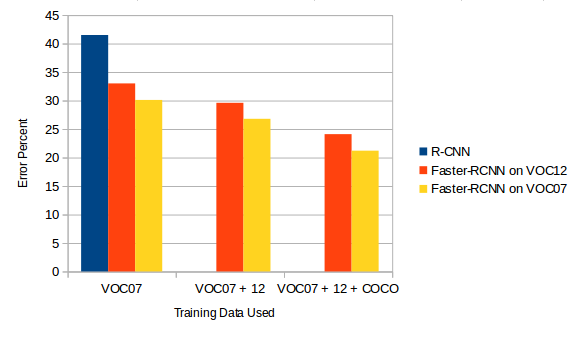
\includegraphics[width=14cm]{figs/data_vs_error.png}
\centering
\caption{Improvement of error as data increases, compared to error improvements due to algorithm improvements.
As we can see by comparing the drop from RCNN to Faster-RCNN on VOC07 only, and the drop from adding training data to Faster-RCNN, increasing data contributes significantly to error reduction.}
\end{figure}

Therefore, for real-world application development, data can be cheaper and more effective than scientists, especially as new tools such as FireCaffe~\cite{firecaffe} allow researchers rapidly train on huge datasets.
This is especially true given the rise of crowdsourcing platforms such as Amazon Mechanical Turk (MTurk) reduces the cost of labor from up to \$20/hr of in-house annotators down to around \$6.
While many existing tools support image classification, like MTurk itself, and some tools support bounding box labeling in images, few tools exist for frame-by-frame labeling in videos.
VATIC~\cite{Vatic} stands out as being one of the best, as it not only makes high quality annotations one of its main goals, but also cost and scalability.

My work borrows and improves upon many concepts and results from VATIC's user studies, but I focus on an additional goal that is extremely important in creating datasets for real applications. That goal is researcher happiness.
Although VATIC extensively tested its ``User Interfaces'', I argue in chapter~\ref{chap:experimenter} that both the annotators and the experimenters are users, and the interfaces should be smooth for both when creating a tool.

In chapter~\ref{chap:annotator}, I discuss my take on VATIC's User Interface principles for the annotator, and improvements upon them.

I also release all related code for BeaverDam, my video labeling platform, on Github.\footnote{http://github.com/antingshen/beaverdam} At time of writing, the library has been used by Berkeley Deep Drive, DeepScale, BMW, and XYSense.

\section*{Related Work}
\label{sec:related}

There are a large number of static image annotators available, used to create the large number of publicly available image datasets.~\cite{IG02}~\cite{LabelMe}~\cite{ImageNet}~\cite{Pascal}
These cannot be used for videos.
For most computer vision applications that only require images instead of videos, these simpler alternatives should be used.
For bounding box annotations, crowdsourcing sites such as Mechanical Turk or Crowdflower may have templates providing static image labeling functionality.
For more complicated labels, tools such as LabelMe~\cite{LabelMe} provide many features for tasks such as image segmentation.
However, these tools were not designed for videos, so annotating a video using these tools would require each frame to be individually labeled, which fails to take advantage of similarity between frames.

There exists some public datasets of labeled videos that use static image annotators.
The YouTube-8M dataset~\cite{YouTube-8M} has millions of annotated videos, but they are annotated using the Inception V3 model trained on ImageNet.
The KITTI dataset~\cite{KITTI}, as well as a dataset being built at Berkeley Deep Drive, have labeled videos.
But these videos are not labeled every frame, instead an image is sampled every few seconds.
Those images are then labeled using static image annotators.
While these types of sampled image datasets are still useful, they don't allow research on supervised learning using nearby frames of a video, such as using an LSTM that uses each frame as input.
Furthermore, for applications such as ADAS where every frame will be available and need to be labeled at inference time, machine learning intuition tells us that having a training dataset to match test time produces better results.

BeaverDam is designed to create frame-by-frame bounding box labeled video datasets.
Existing tools that handle videos include LabelMe video~\cite{LabelMeVideo}, which does arbitrary polygonal annotations using homography preserving linear interpolation.
Another tool, ViPER~\cite{ViPER}, annotates videos but is optimized for spatial labeling.
Few other tools have tackled video annotation~\cite{FlowBoost}~\cite{Agarwala}~\cite{Fisher}~\cite{Smeaton}~\cite{Laptev}.
All of these tools are effective at building large datasets with high quality labels, but they are not necessarily economical and often require high worker ~\cite{AnnotationCost}.
Some inefficiencies come from being too specific to a single type labeling problem and failing to generalize, while others result from inefficiencies in implementation and design.
The best tool we found for our task of labeling bounding boxes in videos is VATIC~\cite{Vatic}, which was created as a better alternative to the other tools cited above, and was used to create a large video dataset~\cite{virat}.

However, labeling videos with VATIC is still difficult and expensive, either due to inefficiencies within the tools.
Even setting up the first job is often a week-long project, consuming valuable researcher time.
Once set up, workers spend a long time labeling objects in the videos due to rough edges in the toolkit.
Modifying them for each dataset's custom specifications is also difficult.
We created BeaverDam to address these problems, while keeping in mind the valuable insights contributed by VATIC.
